\tableofcontents

\newpage

\section{Задание}
По выданному преподавателем варианту разработать и исследовать работу комплекса программ обмена данными в режиме прерывания программы. Основная программа должна изменять содержимое заданной ячейки памяти (Х), которое должно быть представлено как знаковое число. Область допустимых значений изменения Х должна быть ограничена заданной функцией F(X) и конструктивными особенностями регистра данных ВУ (8-ми битное знаковое представление). Программа обработки прерывания должна выводить на ВУ модифицированное значение Х в соответствии с вариантом задания, а также игнорировать все необрабатываемые прерывания.
\begin{figure}[H]
\centering
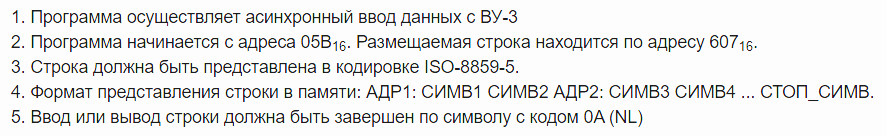
\includegraphics[scale=0.6]{task}
\label{pic:task}
\end{figure}

\section{Текст комплекса программ}
\begin{center}
\begin{tabular}{c}
\begin{lstlisting}[basicstyle=\ttfamily]
	ORG 0x0
V0:	WORD $DEF, 0x180
V1:	WORD $DEF, 0x180
V2:	WORD $INT2, 0x180
V3:	WORD $INT3, 0x180
V4:	WORD $DEF, 0x180
V5:	WORD $DEF, 0x180
V6:	WORD $DEF, 0x180
V7:	WORD $DEF, 0x180
DEF:	IRET

	ORG 0x031
X:	WORD 25
MIN:	WORD -34
MAX:	WORD 29

START:	DI
	LD #0xA
	OUT 5
	LD #0xB
	OUT 7

CYCLE:	HLT	; BREAKPOIN 1
	DI
	LD X
	ADD #3
	CMP MAX
	BLT GROW
	LD MIN
GROW:	ST X
	HLT	; BREAKPOIN 2
	EI
	BR CYCLE
\end{lstlisting}
\end{tabular}
\end{center}

\begin{center}
\begin{tabular}{c}
\begin{lstlisting}[basicstyle=\ttfamily]
INT2:	CLA
	IN 4
	PUSH
	ASL
	ADD &0
	NEG
	ADD $X
	CMP $MIN
	BGE SAVE
	LD $MIN
SAVE:	ST $X
	POP
	IRET

INT3:	LD $X
	ASL
	ASL
	NEG
	SUB #10
	OUT 6
	IRET
\end{lstlisting}
\end{tabular}
\end{center}

\section{Описание комплекса программ}
\subsection{Назначение комплекса программ}
Основная программа увеличивает на 3 содержимое X (ячейки памяти с адресом 0x031) в цикле. Если значение оказывается вне ОДЗ, в X помещается минимальное по ОДЗ число. По нажатию кнопки готовности КВУ-2 обработчик прерывания вычитает утроенное содержимое введенных данных из X, результат записывается в X. По нажатию кнопки готовности КВУ-3 обработчик прерывания осуществляет вывод результата вычисления функции $F(X)=-4X-10$ на КВУ-3.

\subsection{Область представления и область допустимых значений данных}
\subsubsection{Область представления данных}
\noindent Числа X, MIN, MAX: 8-разрядные знаковые целые числа\\
(для хранения в памяти БЭВМ используется расширение знака)\\
Содержимое регистра данных КВУ-2: набор из 8 логических значений

\subsubsection{Область допустимых значений данных}
\noindent ОДЗ X ограничена функцией $F(X)=-4X-10$ и 8-битным знаковым представлением РДВУ-3.\\

\noindent -34 (0xFFDE) $\leqslant$ X $\leqslant$ 29 (0x001D)\\
MIN $=const=$ -34 (0xFFDE)\\
MAX $=const=$ 29 (0x001D)

\subsection{Расположение в памяти ЭВМ}
\noindent Основная программа: 034\ldots043\\
Обработчик прерывания КВУ-2: 044\ldots050\\
Обработчик прерывания КВУ-3: 051\ldots057\\
Обработчик прерывания по умолчанию: 010\\

\noindent Адрес переменной: 031 (X)\\
Адрес минимального значения переменной: 032 (MIN)\\
Адрес максимального значения переменной: 033 (MAX)

\subsection{Адреса первой и последней выполняемой команд основной программы}
\noindent Адрес первой команды основной программы: 034\\

\section{Методика проверки}
X = 25 (0x0019), MIN = -34 (0xFFDE), MAX = 29 (0x001D)
\begin{enumerate}
\item Загрузить исходные данные и комплекс программ в пямять БЭВМ.
\item Убедиться, что по адресу 039 и 041 установлены точки останова - HLT.
\item Запустить основную программу в режиме работы с адреса 034 и дождаться останова. Программа остановит выполнение перед первой итерацией цикла увеличения переменной X.
\item Произвести запуск еще раз, чтобы выполнить увеличение переменной, и еще раз, чтобы остановиться перед следующим циклом.
\item Прочитать значение ячейки X (031) и убедиться, что там находится значение 28 (0x001C).
\item Вернуть в счетчик команд адрес 03A и произвести очередной запуск. Произвести запуск еще раз, чтобы остановиться перед началом следующей итерации цикла.
\item Прочитать значение ячейки X (031) и убедиться, что там находится значение -34 (0xFFDE).
\item Повторить пункт 4 три раза.
\item Прочитать значение ячейки X (031) и убедиться, что там находится значение -25 (0xFFE7).
\item Установить значение 0x02 в регистр данных КВУ-2 и нажать кнопку готовности.
\item Вернуть в счетчик команд адрес 042 и произвести очередной запуск.
\item Прочитать значение ячейки X (031) и убедиться, что там находится значение -31 (0xFFE1).
\item Установить значение 0xFF в регистр данных КВУ-2 и нажать кнопку готовности.
\item Повторить пункт 11.
\item Прочитать значение ячейки X (031) и убедиться, что там находится значение -34 (0xFFDE).
\item Повторить пункт 4.
\item Прочитать значение ячейки X (031) и убедиться, что там находится значение -31 (0xFFE1).
\item Нажать кнопку готовности КВУ-3.
\item Повторить пункт 11.
\item Посмотреть на значение регистра данных КВУ-3 и убедиться, что там находится значение 114 (0x72).
\end{enumerate}

\section{Вывод}
В ходе выполнения данной лабораторной работы я познакомился с работой прерываний в БЭВМ, векторами прерывания и новыми для меня командами - DI, EI, IRET. Эти знания пригодятся мне для дальнейшей работы с БЭВМ и понимания работы современных ЭВМ.
